\documentclass{beamer}
\usepackage[utf8x]{inputenc}
\usepackage{default}
\setbeamertemplate{navigation symbols}{}
\usepackage{graphicx}
\setbeamertemplate{blocks}[rounded][shadow=true]
\setbeamertemplate{bibliography item}[text]
\usetheme{Berlin}
\beamersetuncovermixins{\opaqueness<1>{25}}{\opaqueness<2->{15}}
\setbeamercolor{structure}{fg=violet!40!black}

\begin{document}
\title[META-LIBRARY]{MNNIT META LIBRARY}
\author[\insertframenumber\ of \inserttotalframenumber \hspace{18mm} Mansi,Alka,Saroj
]{\large{Mansi Maheshwari - 2018CA02} \hspace{50mm} \textsc\large{Alka Rani Tigga-2018CA11} \\\textsc\large{Saroj Kumari-2018CA25}}

\institute[CSED, MNNIT Allahabad, Prayagraj] {\includegraphics[height=1.6cm,width=1.7cm]{mnnitLogo.png}
\vspace*{0.5cm}
\\\normalsize{Department of Computer Science \& Engineering,\\ MNNIT Allahabad, Prayagraj - 211004, India}}
%{\date{July 06, 2020}}%

\begin{frame}
\titlepage
\usepackage{fontspec}
\setromanfont{Times New Roman}
\end{frame}
%\begin{frame}
%\movie{Loading Video...}{sm.avi}
%\includemovie[activate=pageopen, width=200pt,height=150pt] {loading video}{sm.swf}
%\includemovie[autoplay,mouse]{1.\textwidth}{5em}{sm.swf}
%\begin{figure}[ht]
%\includemovie[poster,text={\small(Loading Video...)}]{6cm}{4cm}{sm.swf}
%\end{figure}
%\end{frame}


\begin{frame}[allowframebreaks=0.80]\frametitle{Index}
\tableofcontents
\end{frame}

\section{Introduction}
\begin{frame}\frametitle{INTRODUCTION}
 \begin{block}{}
 	\begin{center}
 	{\textrm The  “MNNIT META LIBRARY”  is design to extend the concept of digital library system.} 
 	\end{center} \\
 	{\textrm This application will be very useful for : \begin{itemize}
\item Students : getting online study materials such as notes, papers, e-books and lecture videos.
\item Teachers : sharing their research details as well as uploading their notes, lecture videos, papers and books.
\end{itemize}}
\end{block}
\end{frame}

\section{Objective}
\begin{frame}\frametitle{OBJECTIVE}
\begin{block}{}
	\begin{itemize}
		\item \textrm Students can avail any course material.
		\item \textrm Providing  digital study material.
		\item \textrm Saves time
		\item \textrm Communication platform
       \item \textrm 24 x 7  availability
      \item \textrm No headache of returning the material or missing the due date.
		\item \textrm Students can avail any course material.
		\item \textrm User friendly : more of selection rather than typing.
	\end{itemize}
\end{block}
\end{frame}

\section{Users of MNNIT-META LIBRARY}
\subsection{Users}
\begin{frame}\frametitle{USERS}
\begin{block}{}
	\begin{itemize}
		\item Guest
		\item Student
		\item Teacher
		\item Admin
	\end{itemize}
\end{block}
\end{frame}


\subsection{Use-Case Diagram}
\begin{frame}\frametitle{USE-CASE DIAGRAM}
		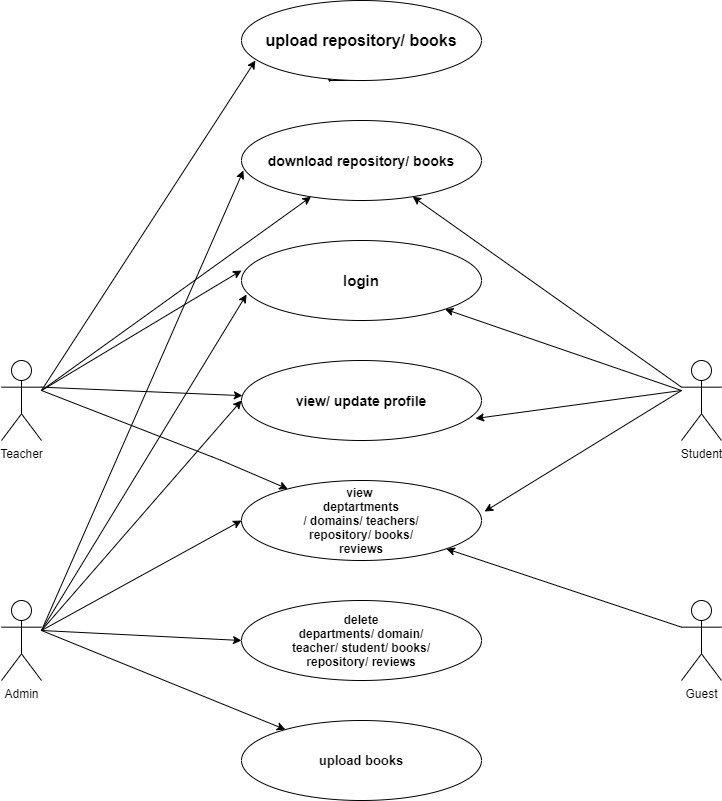
\includegraphics[height=6cm,width=11cm]{usecase_new.png}
\end{frame}

\subsection{ER-Diagram}
\begin{frame}\frametitle{ER DIAGRAM}
		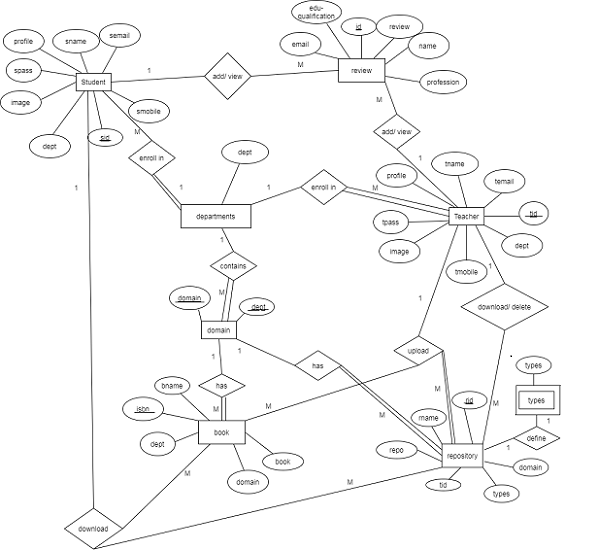
\includegraphics[height=6cm,width=11cm]{er1.png}
\end{frame}

\begin{frame}\frametitle{ER DIAGRAM}
		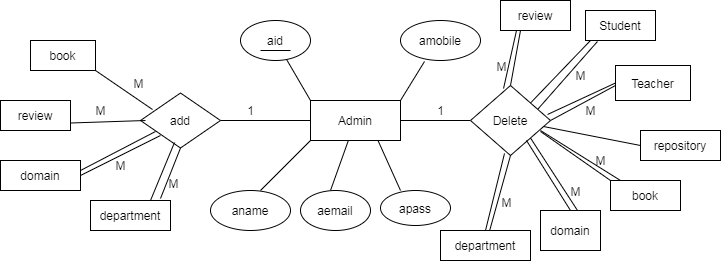
\includegraphics[height=6cm,width=11cm]{er2.png}
\end{frame}


\subsection{Roles}
\subsubsection{Guest}
\begin{frame}\frametitle{GUEST'S ROLE}
\begin{block}{}
	\begin{itemize}
		\item \textrm View :
\begin{itemize}
\item departments
\item subjects
\item faculties Details
\item books
\item notes
\item papers
\item videos
\item reviews
\end{itemize}

		\item \textrm Add their reviews.

	\end{itemize}
\end{block}
\end{frame} 


\subsubsection{Student}
\begin{frame}\frametitle{STUDENT'S ROLE}
\begin{block}{}
\textrm In addition to Guest functionalities : 
	\begin{itemize}
		\item \textrm Create account (mnnit mail id  req.).
		\item \textrm Download : (only after sign in)
\begin{itemize}
\item books
\item notes
\item profile picture
\item papers
\end{itemize}
		\item \textrm Update it's profile info. : (only after sign in)
\begin{itemize}
\item mobile number
\item password
\item profile picture
\item resume
\end{itemize}

	\end{itemize}
\end{block}
\end{frame} 

\subsubsection{Teacher}
\begin{frame}\frametitle{TEACHER'S ROLE}
\begin{block}{}
\textrm In addition to Students functionalities.
	\begin{itemize}
		\item \textrm Upload : (only after sign in)
\begin{itemize}
\item books
\item notes
\item videos
\item papers
\end{itemize}
		\item \textrm Delete : his/her own uploaded material (only after sign in)
\begin{itemize}
\item notes
\item videos
\item papers
\end{itemize}
	\end{itemize}
\end{block}
\end{frame}

\subsubsection{Admin}
\begin{frame}\frametitle{ADMIN'S ROLE}
\begin{block}{}
\textrm \textrm Admin is the supreme authority and is responsible for managing the website.\\
In addition to Guest functionalities.
	\begin{itemize}
		\item \textrm Download : (only after sign in)
\begin{itemize}
\item books
\item notes
\item videos
\item papers
\end{itemize}
		\item \textrm Upload : books (only after sign in)

		\item \textrm Update it's profile info. :
\begin{itemize}
\item mobile number
\item password
\end{itemize}
	\end{itemize}
\end{block}
\end{frame}


\begin{frame}\frametitle{ADMIN'S ROLE}
\begin{block}{}
	\begin{itemize}
		\item \textrm Delete : (only after sign in)
\begin{itemize}
\item departments
\item subjects
\item faculties
\item books
\item notes
\item papers
\item videos
\item reviews
\end{itemize}
	\end{itemize}
\end{block}
\end{frame}




\section{Platforms Used}
    \begin{frame}\frametitle{PLATFORMS USED}
\begin{block}{}
Front End
	\begin{itemize}
		\item JAVA EE 
		\item HTML/CSS/JS
		\item AJAX
		\item JQUERY
	    \item JSP
	    \item BOOTSTRAP
	\end{itemize}
Back End
	\begin{itemize}
	    \item MYSQL
	    \item JDBC (through servlets)
	\end{itemize}
\end{block}
\end{frame}







\section{Screenshots}
\subsection{Home Page}
\begin{frame}\frametitle{HOME PAGE}
		
\includegraphics[height=6cm,width=11cm]{1.png}
\end{frame}


\begin{frame}\frametitle{HOME PAGE}
		
\includegraphics[height=6cm,width=11cm]{3.png}
\end{frame}

\begin{frame}\frametitle{VIEW VIDEOS}
		
\includegraphics[height=6cm,width=11cm]{4.png}
\end{frame}


\begin{frame}\frametitle{SIGN-UP}
		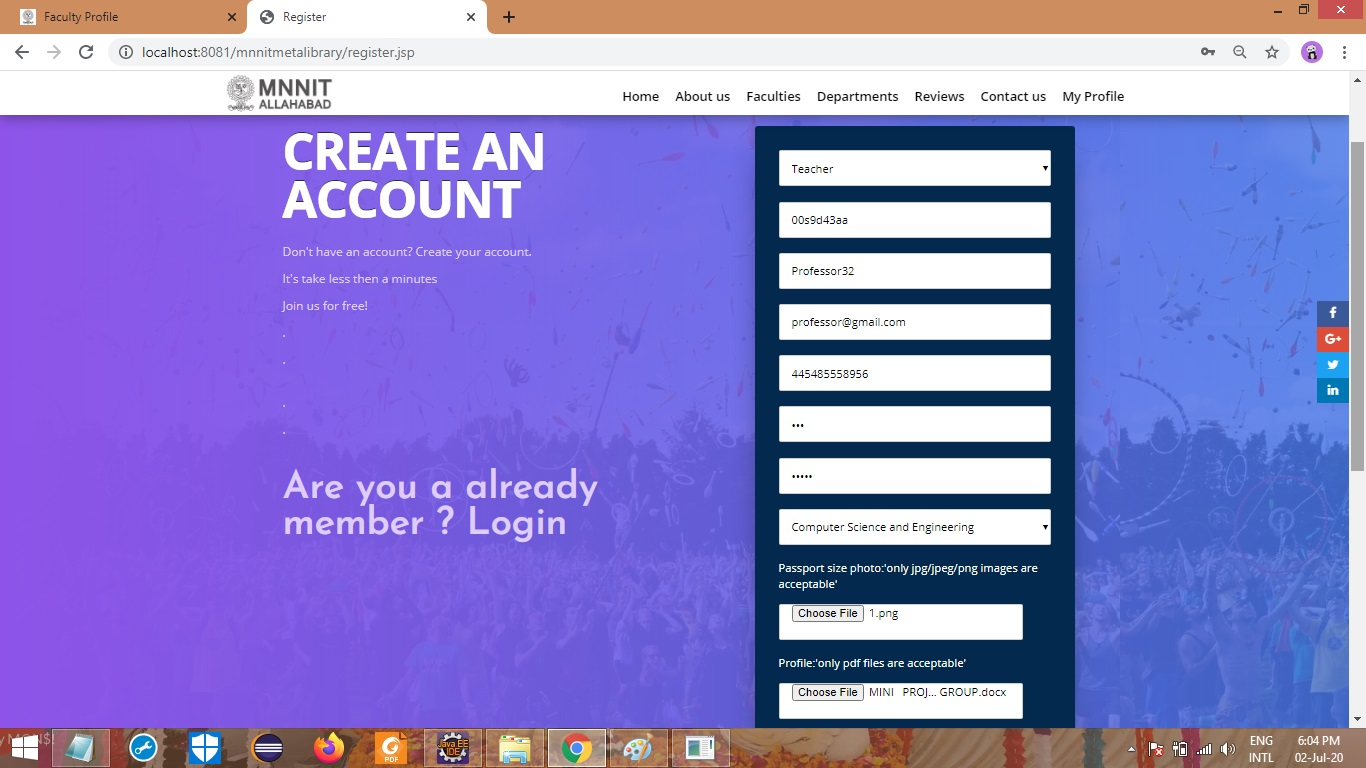
\includegraphics[height=6cm,width=11cm]{13.jpg}
\end{frame}

\begin{frame}\frametitle{SIGN-IN}
		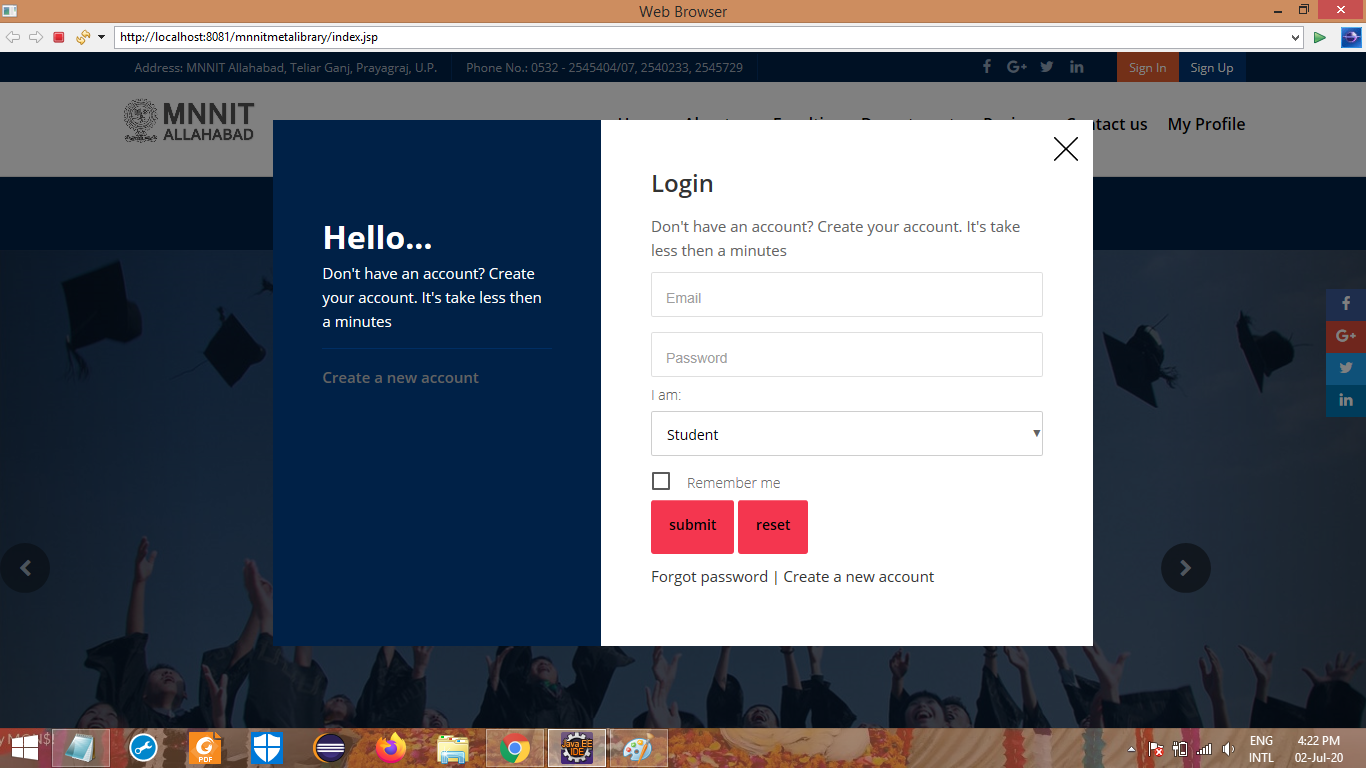
\includegraphics[height=6cm,width=11cm]{5.png}
\end{frame}






\subsection{Student's profile}
\begin{frame}\frametitle{STUDENT'S PROFILE}
		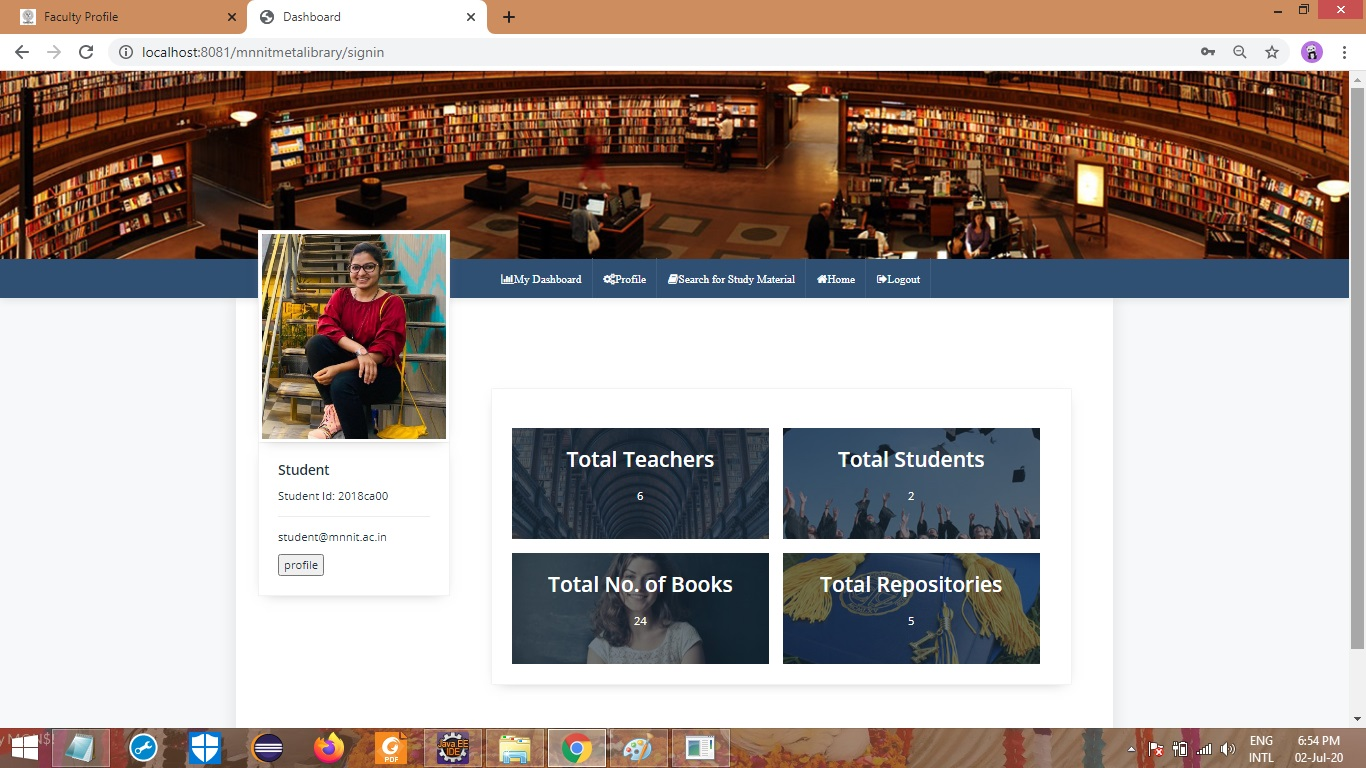
\includegraphics[height=6cm,width=11cm]{s1.jpg}
\end{frame}

\begin{frame}\frametitle{SEARCH STUDY MATERIAL}
		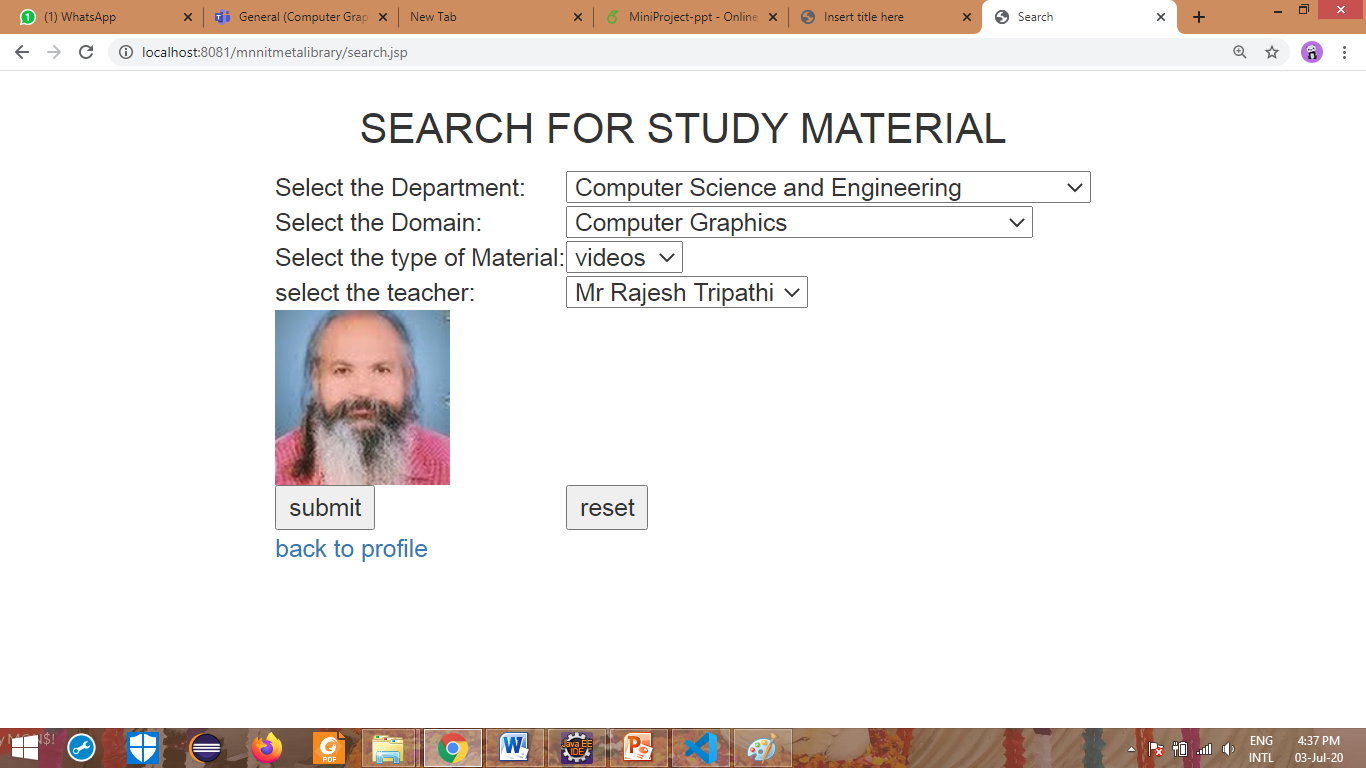
\includegraphics[height=6cm,width=11cm]{s2.png}
\end{frame}

\begin{frame}\frametitle{VIEW / DOWNLOAD STUDY MATERIAL}
		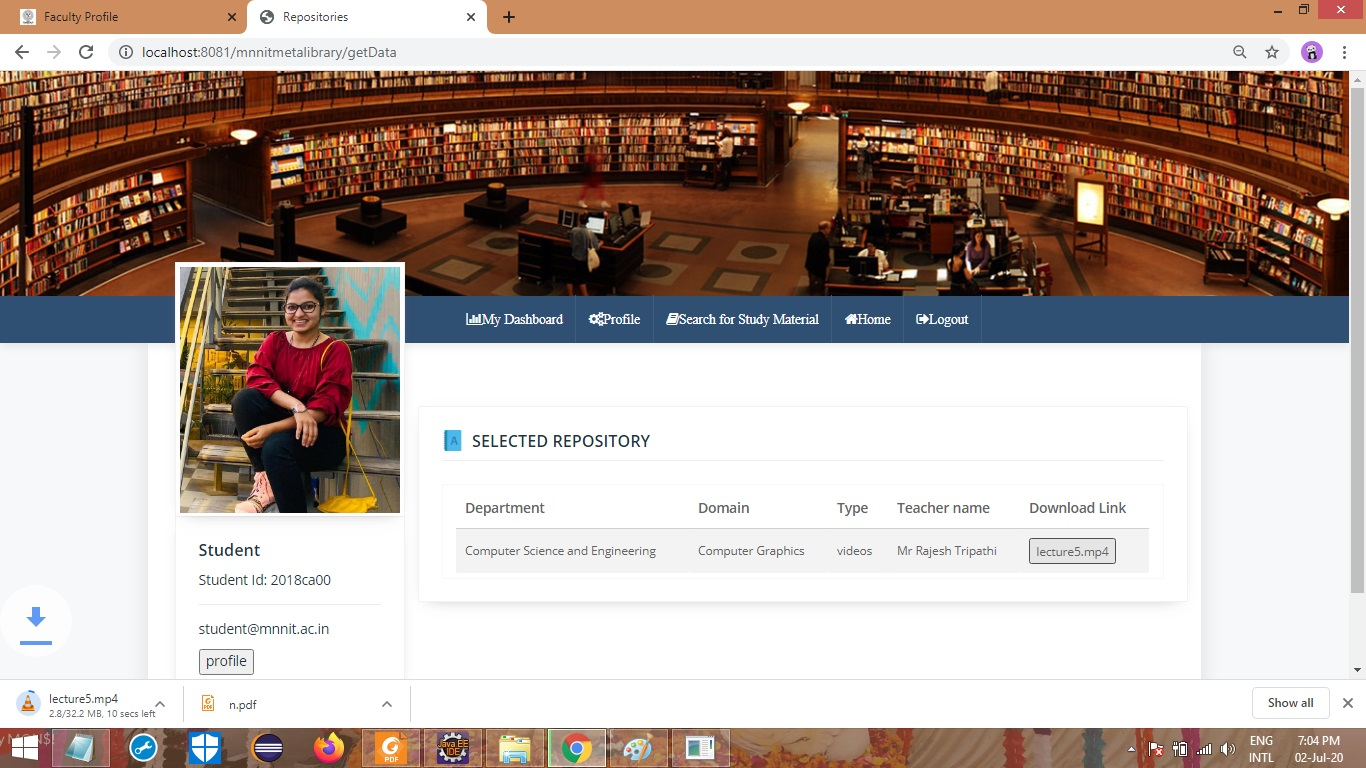
\includegraphics[height=6cm,width=11cm]{s8.jpg}
\end{frame}



\subsection{Teacher's profile}
\begin{frame}\frametitle{TEACHER'S PROFILE}
		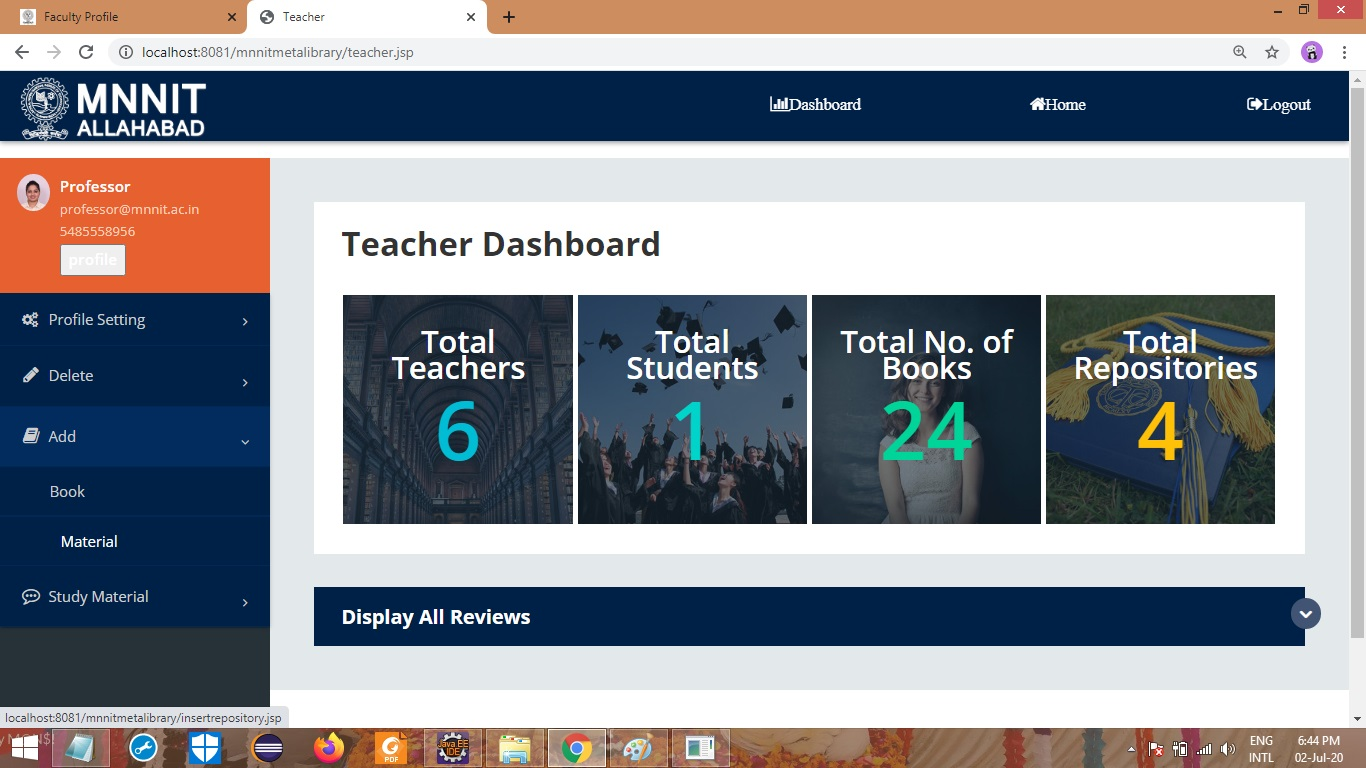
\includegraphics[height=6cm,width=11cm]{t3.jpg}
\end{frame}

\begin{frame}\frametitle{VIEW STUDY MATERIAL}
		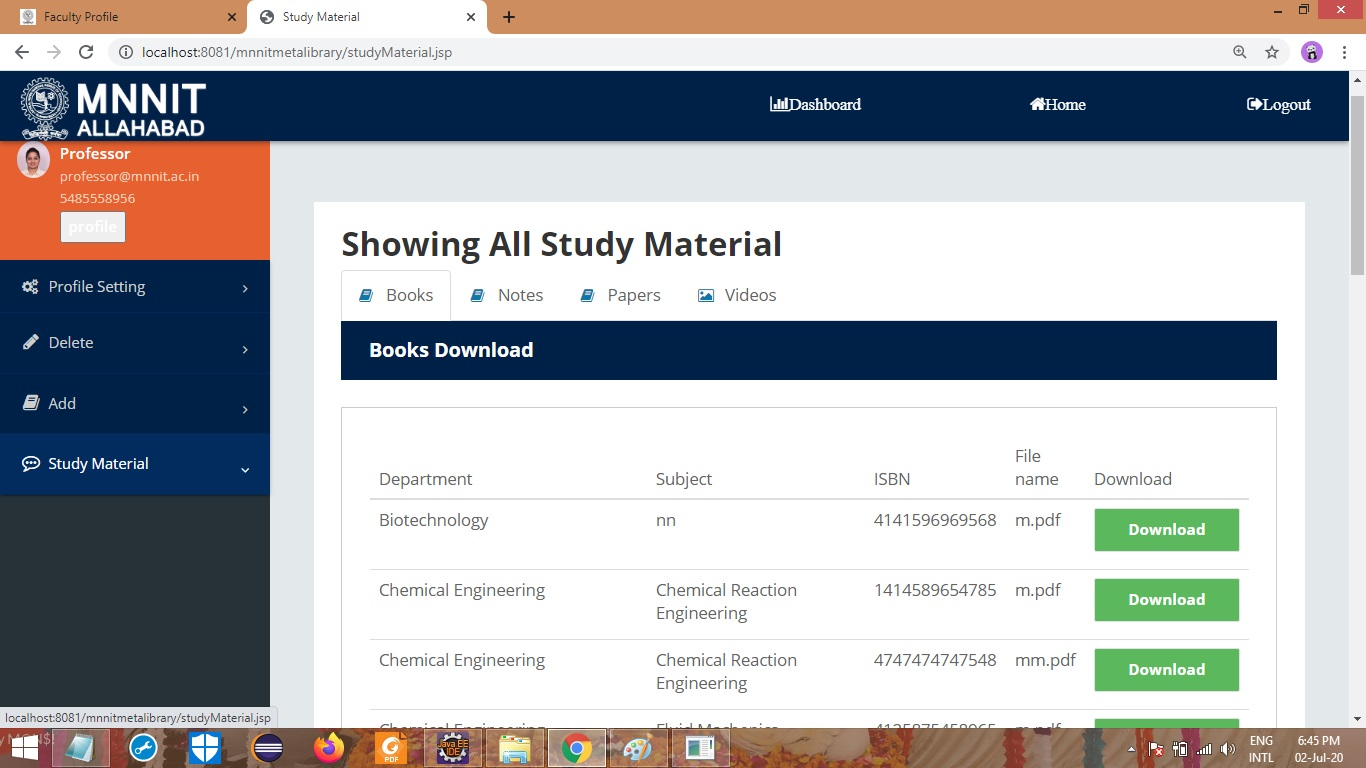
\includegraphics[height=6cm,width=11cm]{t7.jpg}
\end{frame}

\begin{frame}\frametitle{UPLOAD STUDY MATERIAL}
		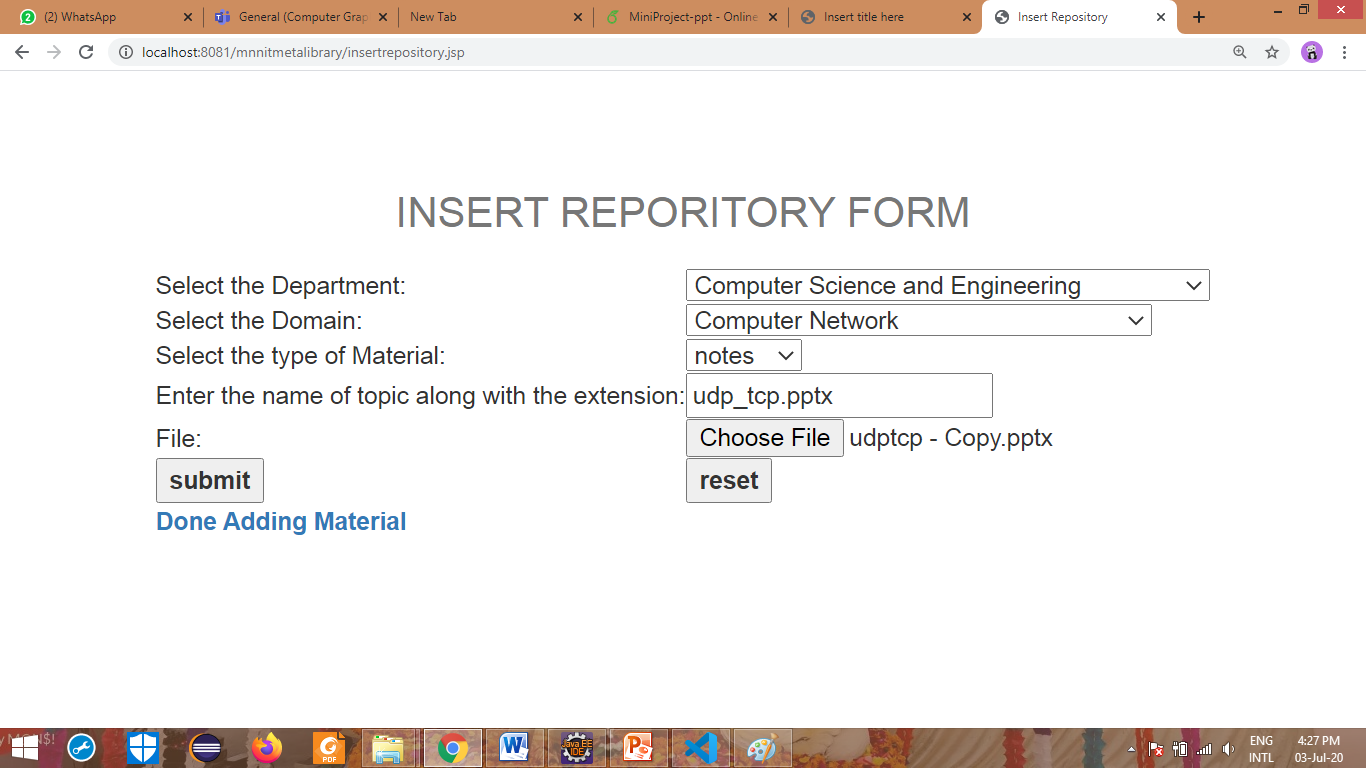
\includegraphics[height=6cm,width=11cm]{t8.png}
\end{frame}



\subsection{Admin's profile}
\begin{frame}\frametitle{ADMIN'S PROFILE}
		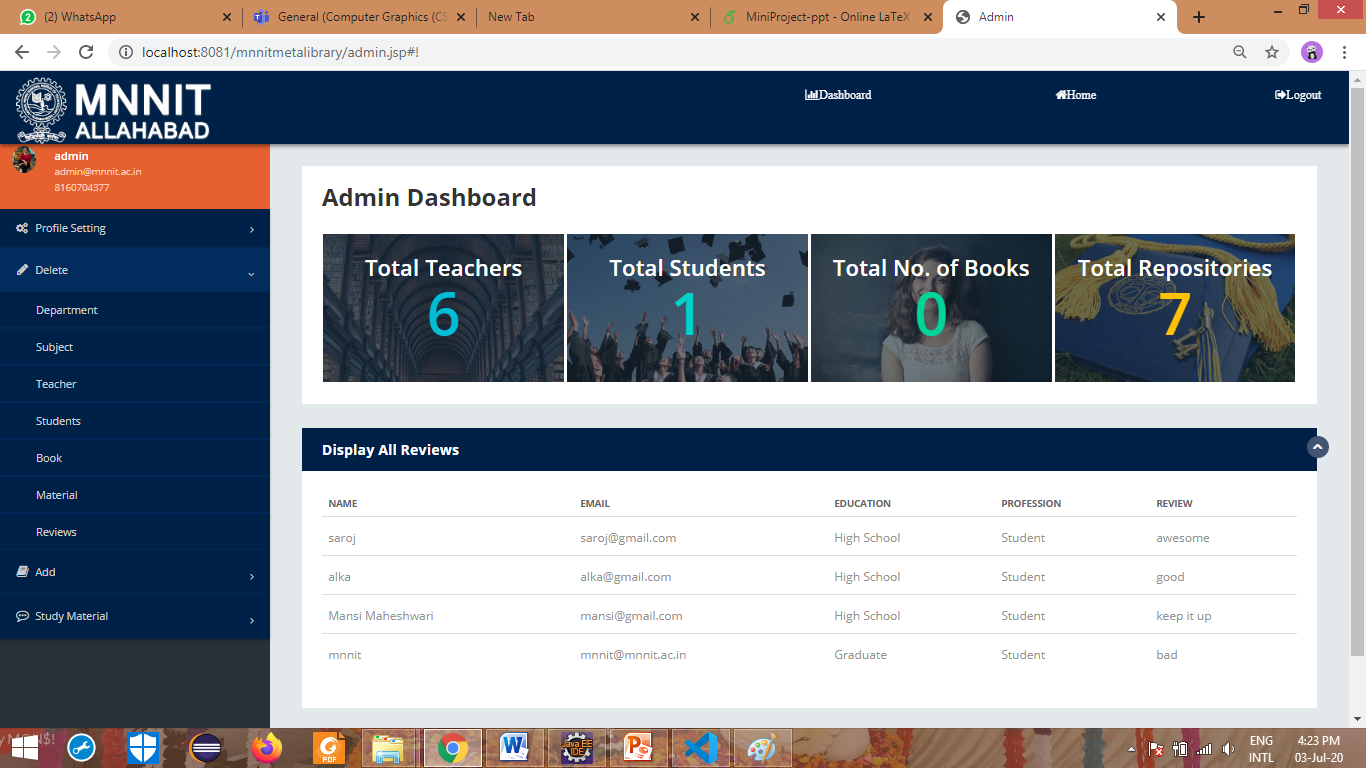
\includegraphics[height=6cm,width=11cm]{a6.png}
\end{frame}

\begin{frame}\frametitle{DELETE DEPARTMENTS}
		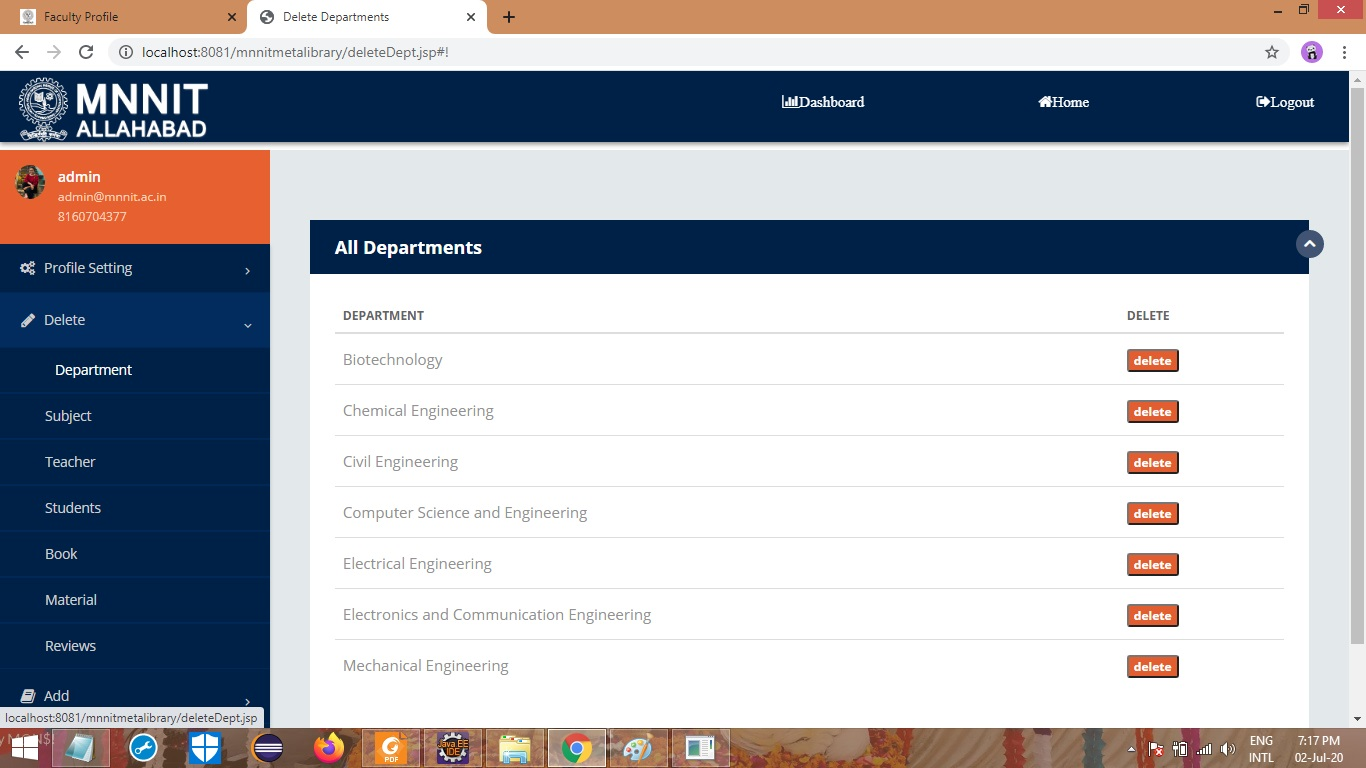
\includegraphics[height=6cm,width=11cm]{a4.jpg}
\end{frame}


\begin{frame}\frametitle{DOWNLOAD STUDY MATERIAL}
		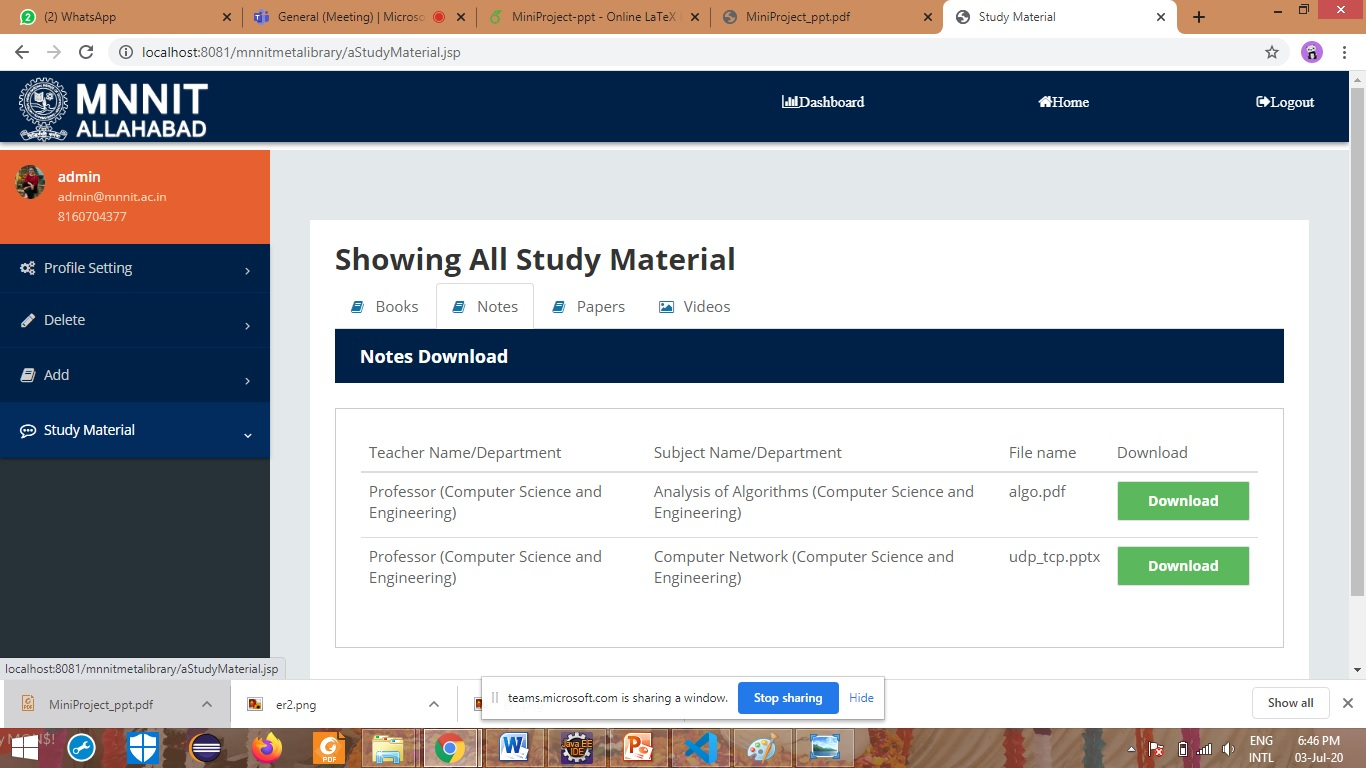
\includegraphics[height=6cm,width=11cm]{a15.jpg}
\end{frame}



\subsection{Home page - tabs}
\begin{frame}\frametitle{VIEW REVIEW}
		
\includegraphics[height=6cm,width=11cm]{11.png}
\end{frame}

\begin{frame}\frametitle{CONTACT US}
		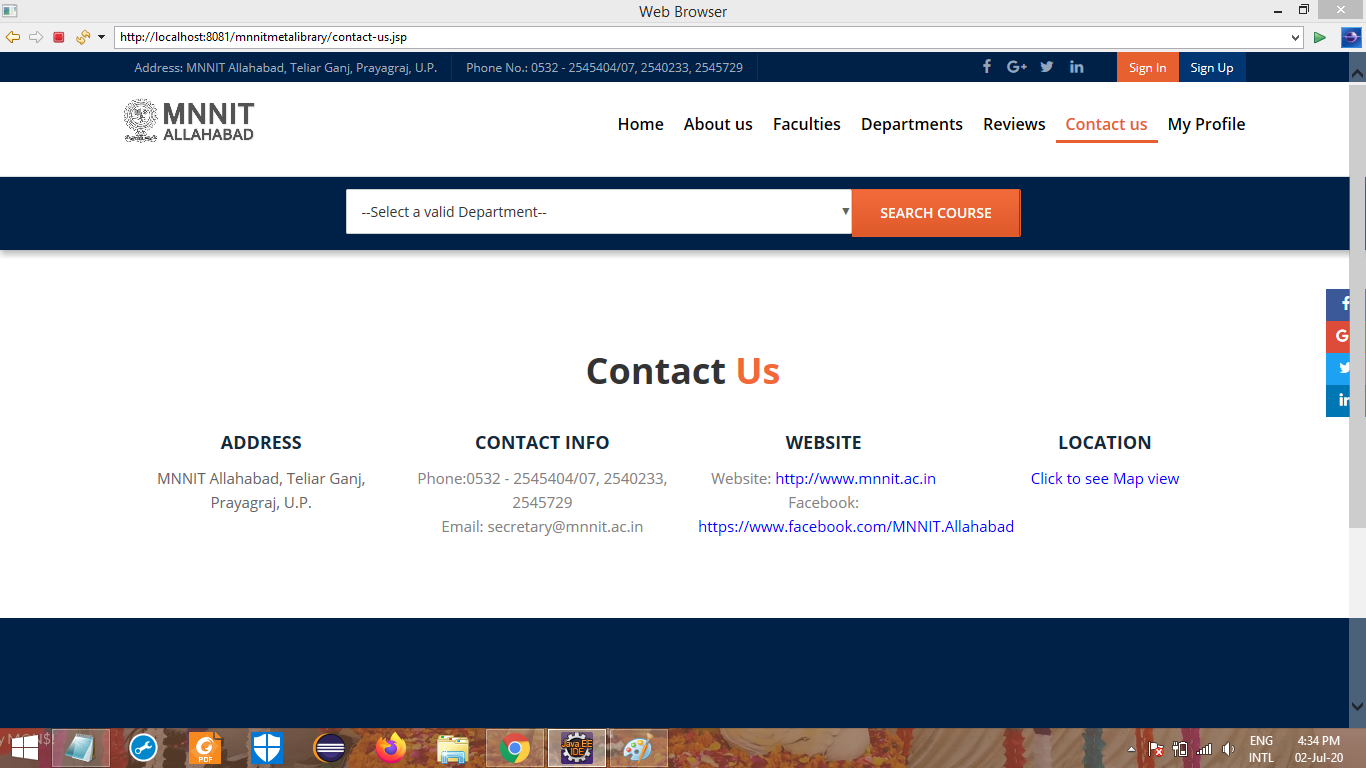
\includegraphics[height=6cm,width=11cm]{12.png}
\end{frame}

\begin{frame}\frametitle{ABOUT US}
		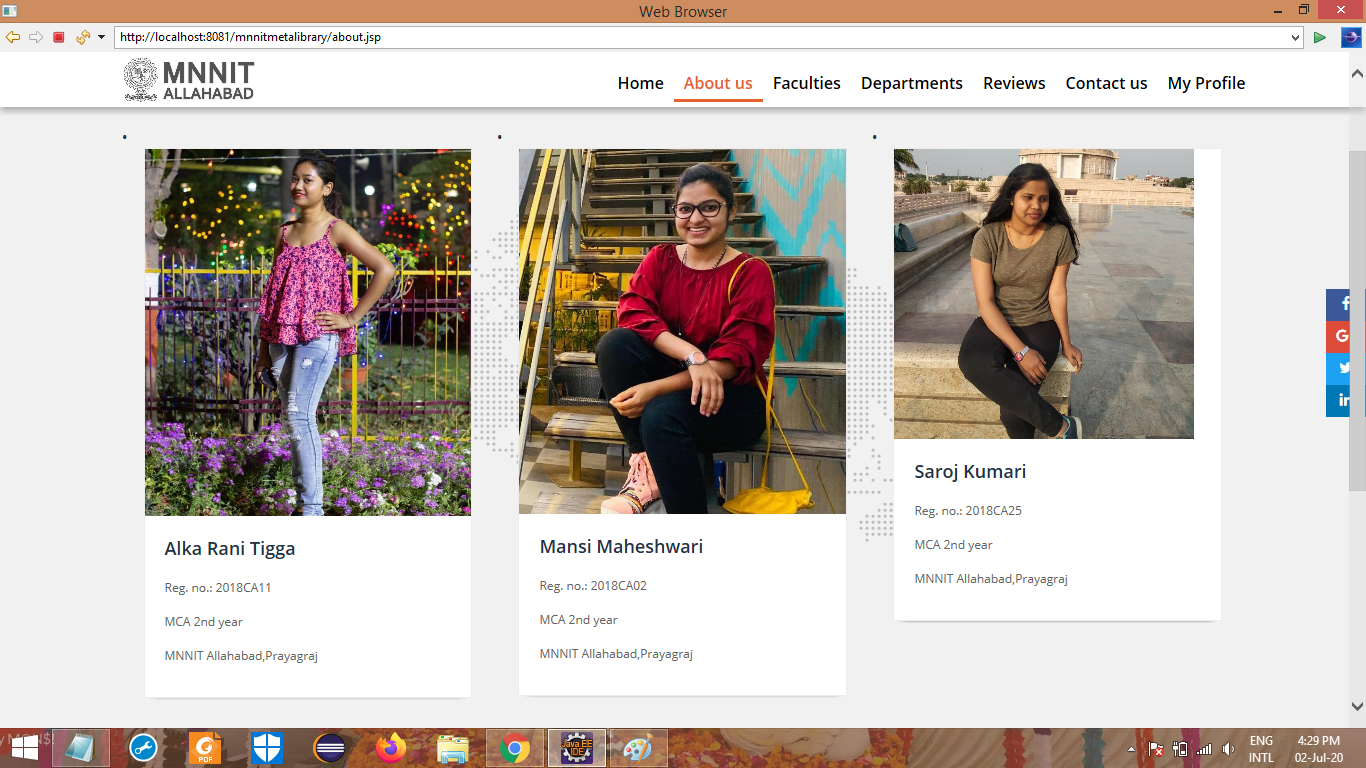
\includegraphics[height=6cm,width=11cm]{last.png}
\end{frame}





\section{Limitations}
\begin{frame}\frametitle{LIMITATIONS}
\begin{block}{}
	\begin{itemize}
		\item \textrm Any substantial enhancement in website will require approval of the administrator.
		\item \textrm Availability of only freely available books.
	\end{itemize}
\end{block}
\end{frame}

\section{Future Scope}
\begin{frame}\frametitle{FUTURE SCOPE}
 \begin{block}{}
\begin{itemize}
    \item Adding secure upload and download functionality for study material.
    \item During sign-up : email verification either through use of API or mailing a randomly generated code to the provided mail.
    \item Extending allowable type of uploading documents to .docx, .ppt, etc. formats.
\end{itemize}
\end{block}
\end{frame}

\section{References}
\begin{frame}\frametitle{References}
\renewcommand{\bibname}{REFERENCES}
\nocite{*}
\bibliography{story}{

\begin{itemize}
    \item https://nalanda.bits-pilani.ac.in/
    \item http://bookboon.com
    \item https://www.free-ebooks.net
\end{itemize}
}
\bibliographystyle{ieeetr} 
\end{frame}

\begin{frame}\frametitle{}
 \begin{block}{}
 	\begin{center} THANK YOU !
 	\end{center} 
\end{block}
\end{frame}

\end{document}
